\documentclass{article}

% Set page size and margins
\usepackage[a4paper,top=2cm,bottom=2cm,left=3cm,right=3cm,marginparwidth=1.75cm]{geometry}
\usepackage[colorlinks=true, allcolors=blue]{hyperref}
\usepackage{tikz}
\usetikzlibrary{positioning}
\usepackage{biblatex}
\addbibresource{aotfmt.bib}
\usepackage{minted}

\title{AOT File Format}
\author{Luca Orlandello}

\begin{document}
\maketitle

\section{Introduction}
The Ahead Of Time (AOT) format is file format for executable, it is not standard, it is used and developed by the WebAssembly Micro Runtime (WAMR) project \cite{WAMR}.
The AOT format is designed to facilitate compilation from a WebAssembly (WASM) module to machine code.
The AOT file format is undocumented, this is not the official documentation but only what i understand reading the WAMR source code (version \verb|2.4.4|, git commit \verb|8c18e3f68b16c4bcaf05996b2636f6ed2b4cf629|).
So there can be bugs or partially correct information in this document.

\subsection{File Format}
The AOT file format decodes in file header and sequence of sections following the grammar \ref{listing:aot-file-grammar}.
Each section consists of a 32-bit unsigned integer section id, a 32-bit unsigned int section length and the actual section contents, whose structure is depended on the section type.
The start of each section must be 4-byte aligned.

\begin{listing}[H]
\begin{minted}{ebnf}
    AOTFile =
        FileHeader,
        TargetInfoSection,
        { CustomSection },
        InitDataSection,
        { CustomSection },
        TextSection,
        { CustomSection },
        FunctionSection,
        { CustomSection },
        ExportSection,
        { CustomSection },
        RelocationSection,
        { CustomSection }
        ;
\end{minted}
\caption{AOT file grammar} 
\label{listing:aot-file-grammar}
\end{listing}

\subsection{How the WAMR compiler generates an AOT file} \label{subsec:how-wasmc-generates-aot}
Before continue some context about how an AOT file is generated by the WAMR compiler, it can be helpful to understand some AOT format design choices.
The WAMR compiler is called \verb|wasmc|, it takes a WASM module as input and produce an AOT file as output.
\verb|wasmc| compile the WASM bytecode (i.e. the content of code section in the WASM module) into LLVM IR, the LLVM IR is further compile down to a relocatable object file.
\verb|wasmc| produce a relocatable ELF object file on a GNU/Linux system and a relocatable COFF object file on Windows.
The relocatable object file, ELF or COFF, is mixed in with the input WASM module to output the AOT file.
%TODO: explain the following line better
In particular the content of target info section, text section and relocation section is taken from the relocatable object file, instead the content of the init data section, function section and export section is taken from the WASM module.
%TODO: check the following line on a virtual machine
So, the content of the target info section, text section, and relocation section in final AOT file may chance depending on whether a ELF or COFF relocatable object file is used.

\medskip
\textbf{Important}: This documentation documents only the AOT file format obtained from a WASM module plus a relocatable ELF object file.


\subsection{Data Representation}
%TODO: little endianess

\section{File Header}

\begin{listing}[H]
\begin{minted}{c}
typedef struct {
        uint8_t    magic[4];
        uint32_t   version;
} FileHeader;
\end{minted}
\caption{AOT file header}
\label{listing:file-header}
\end{listing}

\begin{itemize}
    \item \verb|magic[4]|: A 4 bytes array holding a "magic number", identifying the file as an AOT file.
        \begin{table}[H]
        \centering
        \begin{tabular}{lrl}
            \hline
            Name & Value & Position \\
            \hline
            \verb|MAGIC0| & '\verb|\0|' & \verb|magic[0]| \\
            \verb|MAGIC1| & '\verb|a|'  & \verb|magic[1]| \\
            \verb|MAGIC2| & '\verb|o|'  & \verb|magic[2]| \\
            \verb|MAGIC3| & '\verb|t|'  & \verb|magic[3]| \\
            \hline
        \end{tabular}
        \caption{AOT magic number}
        \end{table}

    \item \verb|version|: This member identifies the AOT file version, the current version is 5.
        The current version is incompatible with the previous versions and it has breaking changes.

        \medskip
        \textbf{Important}: This documentation documents only the AOT file version 5.
\end{itemize}

\section{Target Info Section} \label{sec:target-info}

The target info section has id 0. It decodes into the C struct of listing \ref{listing:target-info}.
The start of the target info section must be 4-byte aligned.

\begin{listing}[H]
\begin{minted}{c}
typedef struct {
        uint16_t   bin_type;
        uint16_t   abi_type;
        uint16_t   e_type;
        uint16_t   e_machine;
        uint32_t   e_version;
        uint32_t   e_flags;
        uint64_t   feature_flags;
        uint64_t   reserved;
        char       arch[16];
} TargetInfo;
\end{minted}
\caption{AOT Target Info Section}
\label{listing:target-info}
\end{listing}

\begin{itemize}
    \item \verb|bin_type|:
        This member identifies from which relocatable object file, ELF or COFF, the content of the target info section, text section and relocation section are taken, see section \ref{subsec:how-wasmc-generates-aot}.
        This member identifies also if the AOT file is targeting a 32-bit or 64-bit architecture and also if the AOT file is targeting a little endian or bit endian machine.

        \begin{table}[H]
        \centering
        \begin{tabular}{lrl}
            \hline
            Name & Value & Meaning \\
            \hline
            \verb|BIN_TYPE_ELF32L| & 0 & ELF,  32-bit, little endian \\
            \verb|BIN_TYPE_ELF32B| & 1 & ELF,  32-bit, big endian \\
            \verb|BIN_TYPE_ELF64L| & 2 & ELF,  64-bit, little endian \\
            \verb|BIN_TYPE_ELF64B| & 3 & ELF,  64-bit, big endian \\
            \verb|BIN_TYPE_COFF32| & 4 & COFF, 32-bit, little endian \\
            \verb|BIN_TYPE_COFF64| & 6 & COFF, 64-bit, little endian \\
            \hline
        \end{tabular}
        \caption{Binary type legal values}
        \label{table:bin-type-legal-value}
        \end{table}

        %TODO: check the following line.
        If the \verb|bin_type| value is \verb|BIN_TYPE_ELF32L| this means that the target info section, text section and relocation section are taken from a relocatable ELF object file with the field \verb|e_ident[EI_CLASS]| set to \verb|ELFCLASS32| and the field \verb|e_ident[EI_DATA]| set to \verb|ELFDATA2LSB|. If the \verb|bin_type| value is \verb|BIN_TYPE_ELF32B|, \verb|BIN_TYPE_ELF64L| or \verb|BIN_TYPE_ELF64B| the value of these two fields change accordingly, see the ELF header section in the ELF documentation \cite{ELF}.

        In the table \ref{table:bin-type-legal-value} all the little endian entry have the first least significant bit set to 0 and all the big endian entry have the first least significant bit set to 1.
        So with \verb|bin_type & 1| you can know if the AOT file is targeting a little endian or big endian machine.
        In the table \ref{table:bin-type-legal-value} all the 32-bit entry have the second least significant bit set to 0 and all the 64-bit entry have the second least significant bit set to 1.
        So with \verb|bin_type & 2| you can know if the AOT file is targeting a 32-bit or 64-bit machine.
        The value 5 in table \ref{table:bin-type-legal-value} is missing for this two reasons.

    \item \verb|abi_type|:
        This member is never used by WAMR, the WAMR compiler set it always to 0.

    \item \verb|e_type|:
        Table \ref{table:e-type-legal-value} contains the possible values for the \verb|e_type| member.
        \begin{enumerate}
            \item \verb|E_TYPE_REL| simply means that the target info section, text section and relocation section are taken from a relocatable object file, see section \ref{subsec:how-wasmc-generates-aot}.
            \item \verb|E_TYPE_XIP| has the same meaning of \verb|E_TYPE_REL| but it also enable the WAMR execution in place feature, see \verb|wasm-micro-runtime/doc/xip.md| in the WAMR repository.
        \end{enumerate}

        \begin{table}[H]
        \centering
        \begin{tabular}{lrl}
            \hline
            Name & Value & Meaning \\
            \hline
            \verb|E_TYPE_REL| & 1 & Relocatable object file \\
            \verb|E_TYPE_XIP| & 4 & Enable execution in place \\
            \hline
        \end{tabular}
        \caption{e\_type legal values}
        \label{table:e-type-legal-value}
        \end{table}

    \item \verb|e_machine|:
        This member specifies the machine instruction set for which the AOT file is intended.
        It indicating the type of machine instruction set that the executable code in the text section is designed to run on. \verb|e_machine| in the AOT target info section has the same meaning of \verb|e_machine| in the ELF header \cite{ELF}.

        \begin{table}[H]
        \centering
        \begin{tabular}{lrl}
            \hline
            Name & Value & Meaning \\
            \hline
            \verb|E_MACHINE_X86_64|       &     62 & AMD x86-64 architecture \\
            \verb|E_MACHINE_WIN_X86_64|   & 0x8664 & Windows x86-64 architecture \\
            \verb|E_MACHINE_386|          &      3 & Intel 80386 \\
            \verb|E_MACHINE_WIN_I386|     &  0x14c & Windows i386 architecture \\
            \verb|E_MACHINE_ARM|          &     40 & ARM 32-bit architecture (AARCH32) \\
            \verb|E_MACHINE_AARCH64|      &    183 & ARM 64-bit architecture (AARCH64) \\
            \verb|E_MACHINE_MIPS|         &      8 & MIPS I Architecture \\
            \verb|E_MACHINE_XTENSA|       &     94 & Tensilica Xtensa Architecture \\
            \verb|E_MACHINE_RISCV|        &    243 & RISC-V 32/64 bit \\
            \verb|E_MACHINE_ARC_COMPACT|  &     93 & ARC International ARCompact \\
            \verb|E_MACHINE_ARC_COMPACT2| &    195 & Synopsys ARCompact V2 \\
            \hline
        \end{tabular}
        \caption{e\_machine values supported by WAMR}
        \label{table:e-machine-legal-values}
        \end{table}

        The difference between \verb|E_MACHINE_X86_64| and \verb|E_MACHINE_WIN_X86_64|, \verb|E_MACHINE_386| and \verb|E_MACHINE_WIN_I386| is due to the difference between ELF and COFF format, see section \ref{subsec:how-wasmc-generates-aot}.
        \verb|E_MACHINE_X86_64| and \verb|E_MACHINE_386| are taken from the \verb|e_machine| field of  an ELF header, instead \verb|E_MACHINE_WIN_X86_64| and \verb|E_MACHINE_WIN_I386| have the same meaning of the non Windows version but they are taken from a COFF header.

    \item \verb|e_version|:
        This member identifies the object file version from witch the target info section, text section and relocation section are taken, see section \ref{subsec:how-wasmc-generates-aot}.

        \begin{table}[H]
        \centering
        \begin{tabular}{lrl}
            \hline
            Name & Value & Meaning \\
            \hline
             \verb|E_VERSION_CURRENT| & 1 & Current version \\
            \hline
        \end{tabular}
        \caption{e\_version legal values}
        \label{table:e-version-legal-values}
        \end{table}

    \item \verb|e_flags|:
        This member holds processor-specific flags.
        \verb|e_flags| in the AOT target info section has the same meaning of \verb|e_flags| in the ELF header \cite{ELF}.
        The legal values of \verb|e_flags| are defined in ABI specification of the machine instruction set. For example see "Chapter 8. ELF Object Files" in RISC-V ABI specification \cite{RISCV-ABI}.
        The \verb|e_flags| member  is never used by WAMR, so you can just put 0.

    \item \verb|feature_flags|:
        This member enable WASM features, each bit of \verb|feature_flags| enable a WASM feature if set to 1.
        If you don't use any WASM feature just put 0.
        The WASM features supported by WAMR are not documented here.

        \medskip
        \textbf{Important}: The activation of some feature flag can change the content of some part of the AOT file format.
        This documentation documents only the AOT file format with \verb|feature_flags| equal to 0.



    \item \verb|reserved|:
        Reserved for future use, just set it to 0.

    \item \verb|arch[16]|:
        Machine architecture name.
        Each machine architecture name must match with the corresponding \verb|e_machine| value.
        Table \ref{table:arch-legal-values} contains the supported \verb|arch| values and the corresponding \verb|e_machine| value.
        \begin{table}[H]
        \centering
        \begin{tabular}{ll}
            \hline
            arch & e\_machine \\
            \hline
            \verb|"x86_64"| & \verb|E_MACHINE_X86_64|, \verb|E_MACHINE_WIN_X86_64| \\
            \verb|"i386"|   & \verb|E_MACHINE_386|, \verb|E_MACHINE_WIN_I386| \\
            \verb|???|      & \verb|E_MACHINE_ARM| \\
            \verb|???|      & \verb|E_MACHINE_AARCH64| \\
            \verb|"mips"|   & \verb|E_MACHINE_MIPS| \\
            \verb|"xtensa"| & \verb|E_MACHINE_XTENSA| \\
            \verb|"riscv"|  & \verb|E_MACHINE_RISCV|\\
            \verb|"arc"|    & \verb|E_MACHINE_ARC_COMPACT|, \verb|E_MACHINE_ARC_COMPACT2| \\
            \hline
        \end{tabular}
        \caption{arch values supported by WAMR}
        \label{table:arch-legal-values}
        \end{table}

        The remaining bytes between the and of the architecture name and the end of the \verb|arch| buffer must be zero.

\end{itemize}

\section{Init Data Section}
The init data section has id 1.
The start of the init data section must be 4-byte aligned.
The init data section decodes in an id, a 32-bit unsigned int section length and sequence of subsections following the grammar \ref{listing:init-data-section-grammar}.
The length of the section is equal to the sum of the lengths of each subsections.
The start of each subsections must be 4-byte aligned.

\begin{listing}[H]
\begin{minted}{ebnf}
    (* The start of the InitDataSection must be 4-byte aligned. *)
    InitDataSection =
        InitDataId,
        u32, (* length of the section in bytes *)
        MemorySubsection,
        TableSubsection,
        TypeSubsection,
        ImportGlobalSubsection,
        GlobalSubsection,
        ImportFunctionSubsection,
        AuxiliarySubsection,
        ObjectDataSubsection
        ;
    InitDataId = "0x01", "0x00", "0x00", "0x00" ;
\end{minted}
\caption{Init data section grammar}
\label{listing:init-data-section-grammar}
\end{listing}

The AOT format is designed to facilitate compilation of a WASM module.
The AOT format is able to facilitate compilation from a WASM module because many parts of an AOT file can be taken directly from the WASM module with few modifications.
Table \ref{table:aot-subsection-wasm-section} summarizes from which section of the WASM form the information of each init data subsection is taken.

\begin{table}[H]
\centering
\begin{tabular}{ll}
    \hline
    Init Data Subsection & WASM Sections \\
    \hline
    Memory          & Memory, Data \\
    Table           & Table, Import \\
    Type            & Type \\
    Import Global   & Import \\
    Global          & Global \\
    Import Function & Import \\
    Auxiliary       & Start, Export, Global \\
    Object Data     & - not taken from the WASM module - \\
    \hline
\end{tabular}
\caption{Mapping between init data subsections and WASM sections}
\label{table:aot-subsection-wasm-section}
\end{table}

\subsection{Memory Subsection}

The content and the structure of the memory subsection is very similar to the memory section of a WASM module and to the data section of a WASM module, see section 5.5.8 and 5.5.14 of the WASM specification \cite{WASM}.
The start of the memory subsection must be 4-byte aligned.
The memory subsection decodes in a vector of WASM memory and in a vector of WASM data segments following the grammar \ref{listing:memory-subsection-grammar}.
A vector of WASM memory is encoded with the 32-bit unsigned int length followed by a sequence of WASM memory.
The vector of WASM memory has always length 1.
A WASM memory is composed of four members in the following order.
\begin{enumerate}
    \item A four byte boolean flag indicating whether a maximum number of memory pages is present, zero means unlimited.
    \item The number of bytes in a memory page.
    \item The initial number of memory pages. The initial number of pages must be always less then or equal to the maximum number of pages.

    \item The maximum number of memory pages. If the four byte boolean flag is 0, the maximum number of pages can be set to 65536.
\end{enumerate}
If the WASM module doesn't have a memory (a WASM module can only have one or zero memory), the WASM Memory members in the AOT module must be filled with these default values, respectively: 0, 65536, 0, 0.
A vector of WASM data segments is encoded with the 32-bit unsigned int length followed by a sequence of WASM data segments.
The initial contents of a memory are zero-valued bytes.
A WASM data segments initialize a range of memory, at a given offset, with a static buffer of bytes.
A WASM data segment is composed of five members in the following order.
\begin{enumerate}
    \item Always zero.
    \item The memory index. This member identifies which memory this data segment initialize. Since there can only be one WASM memory, the memory index is always 0.
    \item The four bytes \verb"0x41 0x00 0x00 0x00".
    \item Offset in the WASM linear memory where this data segment starts.
    \item A buffer of bytes.
\end{enumerate}
If a WASM module has been successfully validated and has no WASM memory, it cannot have WASM data segments.
As a result, this must also apply in an AOT file.

\begin{listing}[H]
\begin{minted}{ebnf}
    (* The start of the MemorySubsection must be 4-byte aligned.
       The first  u32 is always zero.
       The second u32 is the number of WASMMemory elements, it can be only 1.
       The third  u32 is the number of WASMDataSegment elements. *)
    MemorySubsection = u32, u32, WASMMemory, u32, { WASMDataSegment } ;
    WASMMemory =
        u32, (* Boolean flag indicating whether a maximum is present *)
        u32, (* Bytes per page *)
        u32, (* Initial page count *)
        u32  (* Maximum page count *)
        ;
    (* The start of each WASMDataSegment must be 4-byte aligned *)
    WASMDataSegment =
        u32, (* Always 0 *)
        u32, (* Memory index, always 0 *)
        "0x41", "0x00", "0x00", "0x00",
        u32, (* Index in the WASM linear memory where this data segment starts *)
        Buffer
        ;
    (* u32 is the number of bytes *)
    Buffer = u32, { u8 } ;
\end{minted}
\caption{Memory subsection grammar}
\label{listing:memory-subsection-grammar}
\end{listing}

\subsubsection{Memory shrink optimization}
Read section \ref{section:init-data-auxiliary} before this optimization to understand it better.
The WAMR compiler, \verb|wamrc|, preform also the optimization \ref{listing:memory-shrink-optimization} after initializing the WASM memory members in the AOT file as explain before.
The optimization \ref{listing:memory-shrink-optimization} can only be applied if the WASM module has one memory and if there are no \verb|memory.grow| and there are no \verb|memory.size| operations in any function (see section 2.4.4 of the WASM specification \cite{WASM} for \verb|memory.grow| and \verb|memory.size|).
Using optimization \ref{listing:memory-shrink-optimization} the members of the WASM memory in the AOT file are updated.
\begin{listing}[H]
\begin{minted}{c}
bytes_per_page *= initial_page_count;
if (initial_page_count > 0) {
    initial_page_count = 1;
    maximum_page_count = 1;
    uint32_t heap_base;
    /* get_heap_base() can fail if the WASM module is not
    compiled from a C program, see Auxiliary Subsection */
    boolean ok = get_heap_base_linear_memory_index(&heap_base);
    if (ok) {
        bytes_per_page = heap_base;
    }
}
\end{minted}
\caption{Memory shrink optimization}
\label{listing:memory-shrink-optimization}
\end{listing}
Usually a WASM module has a memory of two pages of 64K each, so for linear memory the runtime must allocate an array of 128K in the heap.
On devices with very limited memory, due to external memory fragmentation, you often don't have a contiguous region of 128K of memory in the heap.
The solution to avoid this problem is to shirk the linear memory.
Using the optimization \ref{listing:memory-shrink-optimization} the WAMR compiler tells the WAMR runtime to allocate a contiguous linear memory sufficient to hold only the data section and the stack, see section \ref{section:init-data-auxiliary} and figure \ref{fig:linaer-memory-layout}.
If the WASM module code calls the \verb|malloc|, this \verb|malloc| call "is intercepted" and the required memory is allocated in the heap of the WAMR runtime and not in the WASM linear memory dedicated to the heap.

\subsection{Table Subsection}
The content and the structure of the table subsection is very similar to the table section of a WASM module and to the import section of a WASM module, see section 5.5.7 and 5.5.5 of the WASM specification \cite{WASM}.
The start of the table subsection must be 4-byte aligned.
The table subsection decodes in a vector of imported WASM table and in vector of WASM table following the grammar \ref{listing:table-subsection-grammar}.
A vector of imported WASM table is encoded with the 32-bit unsigned int length followed by a sequence of imported WASM tables.
A vector of WASM table is encoded with the 32-bit unsigned int length followed by a sequence of WASM tables.
This documentations don't documents the structure of a imported WASM table and also don't documents the structure of a WASM table.
It is assumed that the length of the vector of imported WASM table is zero and that the length of the vector of WASM table is zero, so the table subsection consists only of two zero 32-bit unsigned int.

\begin{listing}[H]
\begin{minted}{ebnf}
    (* The start of the TableSubsection must be 4-byte aligned.
       the first  u32 is the length in bytes of the WASMImportTable sequence.
       the second u32 is the length in bytes of the WASMTable sequence. *)
    TableSubsection = u32, { WASMImportTable }, u32, { WASMTable } ;
    WASMImportTable = ; (* not documented *)
    WASMTable = ; (* not documented *)
\end{minted}
\caption{Table subsection grammar}
\label{listing:table-subsection-grammar}
\end{listing}

\subsection{Type Subsection}

The content and the structure of the type subsection is very similar to the type section of a WASM module, see section 5.5.4 of the WASM specification \cite{WASM}.
The start of the type subsection must be 4-byte aligned.
The type subsection decodes in a vector of WASM function type following the grammar \ref{listing:type-subsection-grammar}.
A vector of WASM function type is encoded with the 32-bit unsigned int length followed by a sequence of WASM Function type.
The start of each WASM function type in the vector must be 4-byte aligned.
A WASM function type is composed of four members in the following order.
\begin{itemize}
    \item \verb|TypeFlag|:
        This member is 2 bytes long and can be only zero.
        If some feature flag are enable (see section \ref{sec:target-info}), in the type subsection there may be other types besides WASM function type.
        This member becomes useful to distinguish these types.
    \item 2 bytes identifying the number of parameters of the WASM function type.
    \item 2 bytes identifying the number of return values of the WASM function type.
    \item An array of WASM value type of length equal to the number of parameters plus the number of return values of the WASM function type.
        This array contains the WASM value types corresponding to the WASM function parameters first and then the WASM value types corresponding to the WASM function return values.
        The WASM value types are encoded by a single byte as in table \ref{table:wasm-value-types}.
\end{itemize}

\begin{listing}[H]
\begin{minted}{ebnf}
    (* The start of the TypeSubsection must be 4-byte aligned.
       u32 is the length in bytes of the WASMFuncType sequence. *)
    TypeSubsection = u32, { WASMFuncType } ;
    (* The start of each WASMFuncType must be 4-byte aligned.
       The first  u16 is the number of parameters of the WASM function type.
       The second u16 is the number of return values of the WASM function type *)
    WASMFuncType =  TypeFlag, u16, u16, { WASMValtype } ;
    TypeFlag = "0x00", "0x00" ;
    WASMValtype = "0x7F" | "0x7E" | "0x7D" | "0x7C" ;
\end{minted}
\caption{Type subsection grammar}
\label{listing:type-subsection-grammar}
\end{listing}

\begin{table}[H]
\centering
\begin{tabular}{cl}
    \hline
    WASM value type & Meaning \\
    \hline
    \verb|"0x7F"| & WASM 32-bit integer \\
    \verb|"0x7E"| & WASM 64-bit integer \\
    \verb|"0x7D"| & WASM 32-bit float \\
    \verb|"0x7C"| & WASM 64-bit float \\
    \hline
\end{tabular}
\caption{WASM value types (see sections 2.3.1 and 5.3.1 of the WASM specification \cite{WASM}) }
\label{table:wasm-value-types}
\end{table}

\subsection{Import Global Subsection}
The content and the structure of the import global subsection is very similar to the import section of a WASM module, see section 5.5.5 of the WASM specification \cite{WASM}.
The start of the import global subsection must be 4-byte aligned.
The import global subsection decodes in a vector of imported WASM global variables following the grammar \ref{listing:import-global-subsection-grammar}.
A vector of imported WASM global variables is encoded with the 32-bit unsigned int length followed by a sequence of imported WASM global variables.
This documentations don't documents the structure of a imported WASM global variable.
It is assumed that the length of the vector of imported WASM global variables is zero, so the import global subsection consists of only a zero 32-bit unsigned int.

\begin{listing}[H]
\begin{minted}{ebnf}
    (* The start of the ImportGlobalSubsection must be 4-byte aligned.
       u32 is the length in bytes of the WASMImportGlobal sequence. *)
    ImportGlobalSubsection = u32, { WASMImportGlobal } ;
    WASMImportGlobal = ; (* not documented *)
\end{minted}
\caption{Import global subsection grammar}
\label{listing:import-global-subsection-grammar}
\end{listing}



\subsection{Global Subsection}
The content and the structure of the global subsection is very similar to the global section of a WASM module, see section 5.5.9 of the WASM specification \cite{WASM}.
The start of the global subsection must be 4-byte aligned.
The global subsection decodes in a vector of WASM globals following the grammar \ref{listing:global-subsection-grammar}.
A vector of WASM globals is encoded with the 32-bit unsigned int length followed by a sequence of WASM globals.
The start of each WASM globals in the vector must be 4-byte aligned.
A WASM globals is composed of three members in the following order.
\begin{enumerate}
    \item A WASM value type, the WASM value types are encoded by a single byte as in table \ref{table:wasm-value-types}.
    \item A one byte boolean mutability flag.
    \item A WASM initial expression.
        The start of the WASM initial expression inside the WASM global must be 4-byte aligned.
        A WASM initial expression is a triple consisting of an initial expression type, three zero bytes and the actual initial expression.
        The initial expression type are encoded by a single byte as in table \ref{table:init-expr-type}.
\end{enumerate}

\begin{listing}[H]
\begin{minted}{ebnf}
    (* The start of the GlobalSubsection must be 4-byte aligned.
       u32 is the length in bytes of the WASMGlobal sequence. *)
    GlobalSubsection = u32, { WASMGlobal } ;
    (* The start of each WASMGlobal must be 4-byte aligned *)
    WASMGlobal =  WASMValtype, IsMutable, InitExpr ;
    WASMValtype = "0x7F" | "0x7E" | "0x7D" | "0x7C" ;
    IsMutable = "0x00" | "0x01" ;
    (* The start of each InitExpr must be 4-byte aligned *)
    InitExpr  =
              | "0x41", "0x00", "0x00", "0x00", u32
              | "0x42", "0x00", "0x00", "0x00", i64
              | "0x43", "0x00", "0x00", "0x00", f32
              | "0x44", "0x00", "0x00", "0x00", f64
              | "0x23", "0x00", "0x00", "0x00", u32
              ;
\end{minted}
\caption{Global subsection grammar}
\label{listing:global-subsection-grammar}
\end{listing}


\begin{table}[H]
\centering
\begin{tabular}{cl}
    \hline
    Initial expression type & Meaning \\
    \hline
    \verb|"0x41"| & WASM 32-bit integer constant \\
    \verb|"0x42"| & WASM 64-bit integer constant \\
    \verb|"0x43"| & WASM 32-bit float constant \\
    \verb|"0x44"| & WASM 64-bit float constant \\
    \verb|"0x23"| & index of another WASM globals \\
    \hline
\end{tabular}
\caption{Initial expression type}
\label{table:init-expr-type}
\end{table}

\subsection{Import Function Subsection}
The content and the structure of the import function subsection is very similar to the import section of a WASM module, see section 5.5.5 of the WASM specification \cite{WASM}
The start of the import function subsection must be 4-byte aligned.
The import function subsection decodes in a vector of imported WASM functions.
A vector of imported WASM functions is encoded with the 32-bit unsigned int length followed by a sequence of imported WASM functions.
This documentations don't documents the structure of a imported WASM functions.
It is assumed that the length of the vector of imported WASM functions is zero, so the import functions subsection consists of only a zero 32-bit unsigned int.


\begin{listing}[H]
\begin{minted}{ebnf}
    (* The start of the ImportFunctionSubsection must be 4-byte aligned.
       u32 is the length in bytes of the WASMImportFunction sequence *)
    ImportFunctionSubsection = u32, { WASMImportFunction } ;
    WASMImportFunction = ; (* not documented *)
\end{minted}
\caption{Import function subsection grammar}
\label{listing:import-function-subsection-grammar}
\end{listing}

\subsection{Auxiliary Subsection} \label{section:init-data-auxiliary}
The start of the auxiliary subsection must be 4-byte aligned.
The auxiliary subsection decodes in a tuple following the grammar \ref{listing:auxiliary-subsection-grammar}.

\begin{listing}[H]
\begin{minted}{ebnf}
    (* The start of the AuxiliarySubsection must be 4-byte aligned *)
    AuxiliarySubsection =
        u32, (* Function count *)
        u32, (* Start function index *)
        u32, (* "__data_end" global variable index *)
        u64, (* data end linear memory index *)
        u32, (* "__heap_base" global variable index *)
        u64, (* heap base linear memory index *)
        u32, (* stack pointer global variable index *)
        u64, (* stack pointer linear memory index *)
        u32, (* stack size *)
        
\end{minted}
\caption{Auxiliary subsection grammar}
\label{listing:auxiliary-subsection-grammar}
\end{listing}

\begin{itemize}
    \item Function count: the number of functions.
    \item Start function index: the index of the "main" function, see section 5.5.11 of the WASM specification \cite{WASM}.
\end{itemize}

The remaining seven members of the auxiliary subsection are related to the memory layout, the following paragraphs explain their meaning.
Usually WASM modules are not written by hand, they are compiled from a high level language.
\verb|clang| allows you to compile a C program into a WASM module.
During the compilation from C to WASM \verb|clang| map C memory layout (initialize/uninitialized data, stack and heap) to the WASM linear memory.
Initialize and uninitialized data are mapped to a single data section, not two different sections.
Clang stores in the WASM module in output where the data starts and ends in the WASM linear memory, the stack starts and ends in the WASM linear memory, the heap starts and ends in the WASM linear memory.
These linear memory layout information are store partly in the global section of the WASM module and partly in the export section of the WASM module.
Figure \ref{fig:linaer-memory-layout} summing up the linear memory layout of a WASM module obtained from a C program.
\begin{figure}[!ht]
\centering
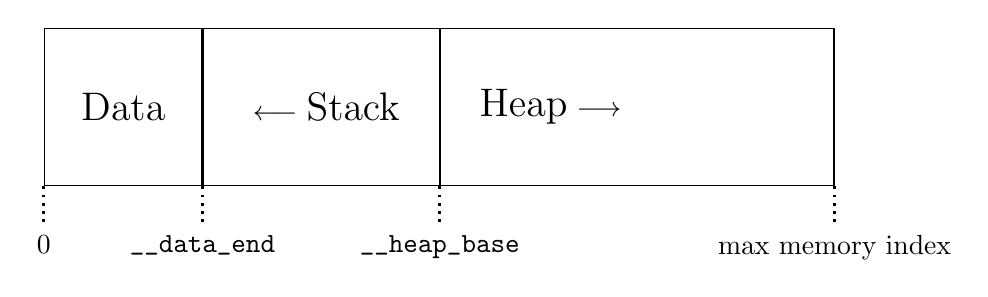
\begin{tikzpicture}[node distance=0]
\node[rectangle, draw=black, minimum width=2cm, minimum height=2cm](data){\Large Data};
\node[rectangle, draw=black, minimum width=3cm, minimum height=2cm, text width=2cm, align=right](stack)[right=of data]{$\longleftarrow$ {\Large Stack}};
\node[rectangle, draw=black, minimum width=5cm, minimum height=2cm, text width=4cm, align=left](heap)[right=of stack]{{\Large Heap} $\longrightarrow$ };

\coordinate (dataBottomLeftCorner) at (data.south west);
\coordinate (dataStartLabel) at ([yshift=-0.5cm] dataBottomLeftCorner);

\coordinate (dataBottomRightCorner) at (data.south east);
\coordinate (dataEndLabel) at ([yshift=-0.5cm] dataBottomRightCorner);

\coordinate (stackBottomRightCorner) at (stack.south east);
\coordinate (heapBaseLabel) at ([yshift=-0.5cm] stackBottomRightCorner);

\coordinate (heapBottomRightCorner) at (heap.south east);
\coordinate (maxMemoryLabel) at ([yshift=-0.5cm] heapBottomRightCorner);

\draw[dotted, line width=1pt] (dataBottomLeftCorner) -- (dataStartLabel);
\node[below] at (dataStartLabel) {0};

\draw[dotted, line width=1pt] (dataBottomRightCorner) -- (dataEndLabel);
\node[below] at (dataEndLabel) {\verb|__data_end|};

\draw[dotted, line width=1pt] (stackBottomRightCorner) -- (heapBaseLabel);
\node[below] at (heapBaseLabel) {\verb|__heap_base|};

\draw[dotted, line width=1pt] (heapBottomRightCorner) -- (maxMemoryLabel);
\node[below] at (maxMemoryLabel) {max memory index};

\end{tikzpicture}
\caption{Linear memory layout of a WASM module compiled from a C program.}
\label{fig:linaer-memory-layout}
\end{figure}
Let's now explain the meaning of the members of the auxiliary subsection from the point of view of someone who is trying to writing a new AOT file starting from a given WASM module.
If you're just trying to read an existing AOT file, you can understand the meaning of the members of the auxiliary subsection by putting yourself in the shoes of a writer.
In order to fill the AOT auxiliary subsection fields with the linear memory layout information, the first to do is to detect if the current WASM module is compiled from a C program\footnote{A programmer can of course write a WASM module by imitating the behavior of a compiler by hand. Let's suppose, for simplicity, that that WASM module is still generated by a compiler.}.

A WASM module is compiled from a C program if there the following three conditions are met:
\begin{enumerate}
    \item There is an exported WASM global variable with the name \verb|"__data_end"|, that exported global variable must be of i32 WASM value type, it must be non mutable and it must be initialized with a WASM 32-bit integer constant.
    \item There is an exported WASM global variable with the name \verb|"__heap_base"|, that exported global variable must be of i32 WASM value type, it must be non mutable and it must be initialized with a WASM 32-bit integer constant.
    \item The initial value of the WASM global variable exported with \verb|"__data_end"| must be less then or equal to the initial value of the WASM global variable exported with \verb|"__heap_base"|.
\end{enumerate}

If the current WASM module is not compile from a C program, fill the AOT auxiliary subsection fields with this default values:
\begin{itemize}
    \item \verb|"__data_end"| global variable index: $2^{32}-1$
    \item Data end linear memory index: 0
    \item \verb|"__heap_base"| global variable index: $2^{32}-1$
    \item Heap base linear memory index: 0
    \item Stack pointer global variable index: $2^{32}-1$
    \item Stack pointer linear memory index: 0
    \item Stack size: 0
\end{itemize}

If a WASM module is compiled from a C program, you can get the WASM linear memory layout information in the following way, see also figure \ref{fig:linaer-memory-layout}.
Data starts at the linear memory index 0.
Data end linear memory index is stored in the WASM global variable exported with the name \verb|"__data_end"|, data start-end interval is open on the end side.
Stack starts at the data end linear memory index.
Stack ends at the heap start linear memory index, stack start-end interval is open on the end side.
Heap start linear memory index is stored in the WASM global variable exported with the name \verb|"__heap_base"|.
Heap end linear memory index is the max memory index.

If the current WASM module is compile from a C program, fill the AOT auxiliary subsection fields ins this way:
\begin{itemize}
    \item \verb|"__data_end"| global variable index: the index of the global variable exported with the name \verb|"__data_end"|.
    \item Data end linear memory index: the initial value of the global variable exported with the name \verb|"__data_end"|.
    \item \verb|"__heap_base"| global variable index: the index of the global variable exported with the name \verb|"__heap_base"|.
    \item Heap base linear memory index: the initial value of the global variable exported with the name \verb|"__heap_base"|
\end{itemize}
The remaining fields to fill are the stack pointer global variable index, the stack pointer linear memory index and the stack size.
If the current WASM module is compile from a C program, you can get the the index of the global variable that hold the stack pointer initial value using the algorithm \ref{listing:get-stack-ptr-global-index}.

\begin{listing}[H]
\begin{minted}{c}
uint32_t get_stack_ptr_global_index(WASMModule *wasm_module,
                                    int32_t heap_base_linear_memory_index) {
    WASMGlobal *g;
    for (uint32_t i = 0; i < w->global_count; i++) {
        g = &wasm_module->globals[i];
        if (g->is_mutable && g->type == WASM_VALTYPE_I32 &&
            g->as.i32 <= heap_base_linear_memory_index) {
            return i;
        }
    }
    return (uint32_t)-1;
}
\end{minted}
\caption{Get the the index of the global variable that hold the stack pointer}
\label{listing:get-stack-ptr-global-index}
\end{listing}

Let \verb|sp_index| the value returned from the function \ref{listing:get-stack-ptr-global-index}.
If \verb|sp_index| is not \verb|-1|:
\begin{itemize}
    \item Stack pointer global variable index: set to \verb|sp_index|.
    \item Stack pointer linear memory index: set to initial value of the global variable of index \verb|sp_index|.
    \item Stack size: (stack pointer linear memory index) - (data end linear memory index).
\end{itemize}
Otherwise if \verb|sp_index| is \verb|-1|:
\begin{itemize}
    \item Stack pointer global variable index: set to \verb|"__heap_base"| global variable index.
    \item Stack pointer linear memory index: set to heap base linear memory index.
    \item Stack size: set to 0.
\end{itemize}



\subsection{Object Data Subsection}
The start of the object data subsection must be 4-byte aligned.
The object data subsection decodes in a vector of object data element following the grammar \ref{listing:object-data-subsection-grammar}.
A vector of object data is encoded with the 32-bit unsigned int length followed by a sequence of object data element.
This documentations don't documents the structure of a object data element.

\begin{listing}[H]
\begin{minted}{ebnf}
    (* The start of the ObjectDataSubsection must be 4-byte aligned.
       u32 is the length in bytes of the ObjectData sequence *)
    ObjectDataSubsection = u32, { ObjectData } ;
    (* The start of each ObjectData must be 2-byte aligned *)
    ObjectData = ; (* not documented *)
\end{minted}
\caption{Object data subsection grammar}
\label{listing:object-data-subsection-grammar}
\end{listing}

\section{Text Section}
\section{Function Section}
The export section has id 3.
The content and the structure of the function subsection is very similar to the function section of a WASM module, see section 5.5.6 of the WASM specification \cite{WASM}.
The start of the export section must be 4-byte aligned.

The init data section decodes in an id and four vector of size equal to the number of functions (see "function count" in section \ref{section:init-data-auxiliary}) following the grammar \ref{listing:function-section-grammar}.
The first vector is a vector of offsets in the text section, the i-th element of the vector is the beginning of the code of the i-th function.
The second vector is a vector of type indexes, the i-th element of the vector means that the i-th function has the i-th type in the vector of types in the type subsection of init data.
The elements of the third and fourth vectors are always zero.

\begin{listing}[H]
\begin{minted}{ebnf}
    (* The start of the FunctionSection must be 4-byte aligned. *)
    FunctionSection =
        FunctionId,
        { u32 }, (* offset in the text section *)
        { u32 }, (* type index *)
        { u32 }, (* Always zero *)
        { u32 }, (* Always zero *)
        ;
    FunctionId = "0x03", "0x00", "0x00", "0x00" ;
\end{minted}
\caption{Function section grammar}
\label{listing:function-section-grammar}
\end{listing}


\section{Export Section}
The export section has id 4.
The content and the structure of the export subsection is very similar to the export section of a WASM module, see section 5.5.10 of the WASM specification \cite{WASM}.
The start of the export section must be 4-byte aligned.
The export section decodes in an id, a 32-bit unsigned int section length and a vector of WASM export element following the grammar \ref{listing:export-section-grammar}.
A vector of WASM exports is encoded with the 32-bit unsigned int length followed
by a sequence of WASM exports.
The start of each WASM export in the vector must be 4-byte aligned.
A WASM export is composed of three members in the following order.
\begin{itemize}
    \item An export index, see section 5.5.10 of the WASM specification \cite{WASM}.
    \item An export description, see section 5.5.10 of the WASM specification \cite{WASM}.
    \item A string, the start of each string must be 2-byte aligned (not 4-byte).
        A string is encoded with 16-bit unsigned int length followed by a sequence of bytes terminated with a zero byte.
        The length of the string include also the final zero byte.
\end{itemize}

\begin{listing}[H]
\begin{minted}{ebnf}
    (* The start of the ExportSection must be 4-byte aligned. *)
    ExportSection =
        ExportId,
        u32, (* length of the section in bytes *)
        u32, (* The number of WASMExport elements *)
        { WASMExport }
        ;
    ExportId = "0x04", "0x00", "0x00", "0x00" ;
    (* The start of each WASMExport must be 4-byte aligned *)
    WASMExport =
        u32, (* Export index *)
        u8, (* Export description *)
        String
        ;
    (* u16 is the number of bytes of the string including the final zero byte.
       The start of each String must be 2-byte aligned. *)
    String = u16, { u8 }, "0x00" ;

\end{minted}
\caption{Export section grammar}
\label{listing:export-section-grammar}
\end{listing}

\section{Relocation Section}

\newpage

\printbibliography

\end{document}
